\documentclass[a4paper,12pt]{extarticle}
\usepackage{geometry}
\usepackage[T1]{fontenc}
\usepackage[utf8]{inputenc}
\usepackage[english,russian]{babel}
\usepackage{amsmath}
\usepackage{amsthm}
\usepackage{amssymb}
\usepackage{fancyhdr}
\usepackage{setspace}
\usepackage{graphicx}
\usepackage{colortbl}
\usepackage{tikz}
\usepackage{pgf}
\usepackage{subcaption}
\usepackage{listings}
\usepackage{indentfirst}
\usepackage{dsfont}
\usepackage[
backend=biber,
style=numeric,
maxbibnames=99
]{biblatex}
\addbibresource{refs.bib}
\usepackage[colorlinks,citecolor=blue,linkcolor=blue,bookmarks=false,hypertexnames=true, urlcolor=blue]{hyperref} 
\usepackage{indentfirst}
\usepackage{mathtools}
\usepackage{booktabs}
\usepackage[flushleft]{threeparttable}
\usepackage{tablefootnote}

\usepackage{chngcntr} % нумерация графиков и таблиц по секциям
\counterwithin{table}{section}
\counterwithin{figure}{section}

\graphicspath{{graphics/}}%путь к рисункам

\makeatletter
% \renewcommand{\@biblabel}[1]{#1.} % Заменяем библиографию с квадратных скобок на точку:
\makeatother

\geometry{left=2.5cm}% левое поле
\geometry{right=1.0cm}% правое поле
\geometry{top=2.0cm}% верхнее поле
\geometry{bottom=2.0cm}% нижнее поле
\setlength{\parindent}{1.25cm}
\renewcommand{\baselinestretch}{1.5} % междустрочный интервал


\newcommand{\bibref}[3]{\hyperlink{#1}{#2 (#3)}} % biblabel, authors, year
\newcommand{\defeq}{\stackrel{\text{def}}{=}}
\addto\captionsrussian{\def\refname{Список литературы (или источников)}} 

\renewcommand{\theenumi}{\arabic{enumi}}% Меняем везде перечисления на цифра.цифра
\renewcommand{\labelenumi}{\arabic{enumi}}% Меняем везде перечисления на цифра.цифра
\renewcommand{\theenumii}{.\arabic{enumii}}% Меняем везде перечисления на цифра.цифра
\renewcommand{\labelenumii}{\arabic{enumi}.\arabic{enumii}.}% Меняем везде перечисления на цифра.цифра
\renewcommand{\theenumiii}{.\arabic{enumiii}}% Меняем везде перечисления на цифра.цифра
\renewcommand{\labelenumiii}{\arabic{enumi}.\arabic{enumii}.\arabic{enumiii}.}% Меняем везде перечисления на цифра.цифра

\begin{document}
\begin{titlepage}
\newpage

{\setstretch{1.0}
\begin{center}
ПРАВИТЕЛЬСТВО РОССИЙСКОЙ ФЕДЕРАЦИИ\\
ФГАОУ ВО НАЦИОНАЛЬНЫЙ ИССЛЕДОВАТЕЛЬСКИЙ УНИВЕРСИТЕТ\\
«ВЫСШАЯ ШКОЛА ЭКОНОМИКИ»
\\
\bigskip
Факультет компьютерных наук\\
Образовательная программа «Прикладная математика и информатика»
\end{center}
}

\vspace{2em}
УДК 004.8 % УДК нужно указывать только для исследовательсвого проекта - удалите эту строку для программного проекта
\vspace{5em}

\begin{center}
%Выберите какой у вас проект
{\bf Отчет об исследовательском проекте на тему:}\\
%{\bf Отчет о программном проекте на тему:}\\
{\bf Кластеризация аудио}\\
(промежуточный, этап 1)
\end{center}

\vspace{2em}

{\bf Выполнил студент: \vspace{2mm}}

{\setstretch{1.1}
\begin{tabular}{l@{\hskip 1.5cm}l}
группы \#БПМИ213 & Бонич Дмитрий Сергеевич 
\end{tabular}}

\vspace{1em}
{\bf Принял руководитель проекта: \vspace{2mm}}

{\setstretch{1.1}
\begin{tabular}{l}
Сендерович Александра Леонидовна\\
Научный сотрудник\\
Факультет компьютерных наук НИУ ВШЭ 
\end{tabular}}

\vspace{\fill}

\begin{center}
Москва 2024
\end{center}

\end{titlepage}
% это титульный лист - выберите подходящий вам из имеющихся в проекте вариантов
\newpage
\setcounter{page}{2}

{
	\hypersetup{linkcolor=black}
	\tableofcontents
}

\newpage

\newpage
\section*{Аннотация}   % this is how to use russian
    Существующие методы глубинного обучения для кластеризации 
    изображений работают довольно хорошо. Однако вопрос качественной
    кластеризации аудио остается открытым. В этой работе мы планируем
    адаптировать лучшие методы кластеризации изображений для 
    задачи кластеризации аудио.

\addcontentsline{toc}{section}{Аннотация}

\section*{Ключевые слова}
Глубинное обучение, обучение без учителя, кластеризация
\pagebreak

\section{Введение}

\subsection{Постановка задачи}

В задаче классификации мы имеем обучающую выборку, где для каждого объекта
известен его класс и от нас требуется моделировать распределение
классов на пространстве объектов. Задача кластеризации более сложная
-- необходимо разбить объекты на осмысленные группы, не зная ни 
самих групп, ни их распределения.

\subsection{Метрики качества}

Чтобы замерить качество кластеризации, как правило, метод
решает задачу на размеченном для кластеризации датасете, 
разумеется, не используя метки классов. Полученные после 
кластеризации номера кластеров будем называть \textit{псевдометками}.
Псевдометки сравниваются с настоящими метками,
и качество определяется как некоторый вид корреляции между ними.

Одной из самых популярных метрик качества является NMI(Normalized Mutual \\
Information).
Пусть у нас есть пара случайных величин $X$ и $Y$, тогда:

\[
	\text{NMI}(X,Y) = \frac{\text{KL}(p_{(X, Y)}| p_X \cdot p_Y)}{\sqrt{H(X)H(Y)}}
\]
Тут KL это Кульбака-Лейблера, H -- энтропия.
При подсчете NMI мы считаем распределения меток и псевдометок 
за $X$ и $Y$, и вычисляем \textit{оценку максимального правдоподобия}\footnote{далее ОМП}. NMI 
принимает значения от 0 до 1.

Еще одной используемой метрикой является ARI(Adjusted Rand Index).
Это скорректированная версия метрики RI (Rand Index) \cite{rand1971objective}.
Определяется ARI следующим образом:

\[
	\text{ARI}(X, Y) = \frac{\text{RI}(X, Y) - \mathds{E}[\text{RI}(X, Y)]}{1 - \mathds{E}[\text{RI}(X, Y)]}
\]

ARI принимает значения от 0 до 1.

Также в качестве метрики качества можно использовать долю 
правильных ответов, как и в задаче классификации. Однако предварительно 
необходимо решить \textit{задачу о назначениях}\footnote{\url{https://en.wikipedia.org/wiki/Assignment_problem}}
между псевдометками и метками.
Мы переименуем псевдометки так, чтобы достичь максимального качества.
Затем на переименованных псевдометках мы посчитаем долю правильных ответов, которую 
и используем в качестве метрики качества.

\subsection{Классические методы решения}

С точки зрения классических методов кластеризуемые
объекты это точки в многомерном пространстве. Такие
методы обычно имеют итерационную природу и решают 
задачу выделения кластеров точек, находя их скопления, 
области с повышенной плотностью, некоторые структуры.
Приведем пример такого метода.

\subsubsection{K-means}

Одним из самых простых и известных методов является
K-means. Он работает на базе EM-алгоритма \cite{dempster1977maximum}.
K-means итерационно пытается найти два неизвестных набора переменных ---
номера кластеров для объектов и центры этих кластеров. 
Количество кластеров фиксировано и задается до начала 
работы алгоритма в качестве гиперпараметра $k$.

В начале своей работы классический K-means инициализирует все 
центры кластеров случайно. Затем чередуются E и M шаги до 
сходимости. На E-шаге мы назначаем каждому объекту номер
кластера, к центру которого объект ближе всего в качестве псевдометки.
На M-шаге мы вычисляем ОМП для каждого центра кластера, то есть 
берем в качестве центра кластера усредненную точку из всех объектов 
с псевдометкой этого кластера.

\section{Обзор литературы}

При кластеризации сложных объектов, таких как изображения или 
аудио, недостаточно вытянуть данные объекта в вектор и применить
классический алгоритм кластеризации для полученных точек. 
Чтобы алгоритмы кластеризации хорошо работали, входное 
пространство точек должно обладать некоторыми свойствами.
В идеале, близкие в этом пространстве точки должны принадлежать 
к одной группе.

Таким образом, задачу кластеризации сложных объектов можно 
разделить на две части: получение представлений объектов 
образующих пригодное для кластеризации пространство точек, и 
сама кластеризация этих представлений. Метод, переводящий объекты
в признаки, будем называть \textit{энкодером}.

\subsection{DeepCluster}

Одним из первых методов использующих глубинное обучение для 
кластеризации изображений, был
DeepCluster \cite{Caron_2018_ECCV}. DeepCluster использует 
сверточную нейросеть $f_\theta$ в качестве энкодера.
К полученным признакам применяется K-means, и мы получаем
псевдометку $y_n$ для каждого изображения $x_n$. Затем к 
сверточной сети прикрепляется
классификационная голова $g_W$. $g_W$ предсказывает 
вероятности кластеров для объекта по его признакам,
полученным из $f_\theta$. Псевдометки используются как настоящие для подсчета логистической 
функции потерь. Таким образом, мы решаем следующую задачу 
оптимизации:

\[
	\min_{\theta, W} \frac{1}{N}\sum_{n=1}^N 
	l(g_W(f_\theta(x_n)), y_n)
\]

Здесь $N$ -- это размер батча, $l$ -- логистическая 
мультиномиальная функция потерь

По усредненному значению функции потерь для батча делается проход назад, и веса 
$\theta$ и $W$ обновляются стохастическим градиентным спуском. Затем 
шаги кластеризации и оптимизации параметров сети повторяются 
заданное количество эпох.

Однако в такой постановке метод выраждается в тривиальные 
решения. Их существует 2 типа -- пустые кластеры и 
тривиальная параметризация

Чтобы не допустить возникновения пустых кластеров 
сделаем следующую модификацию K-means. Пусть 
на некоторой итерации у нас появился пустой 
класс A. Тогда возьмем случайный непустой класс 
B. Добавим к центру B шум, получив новый центр 
для кластера A. Переназначим классы точек из B 
так, чтобы каждая точка имела класс ближайшего 
центра кластера. 

Тривиальная параметризация возникает, когда 
распределение классов становится сильно неравномерным. 
Тогда классификационной голове становится выгодно выдавать 
только несколько наиболее часто встречающихся классов, игнорируя остальные. 
Чтобы этого избежать, необходимо сэмплировать объекты для батча 
из равномерного распределения по псевдометкам с предыдущего шага.

\subsection{SPICE}

SPICE предложенный в \cite{niu2021spice}, является более 
продвинутым методом по сравнению с DeepCluster и имеет лучшее качество.
Целью SPICE является обучение энкодера и кластеризационной головы. 
В качестве энкодера используется сверточная нейросеть.
Кластеризационная голова это двухслойный MLP(Multilayer perceptron). 
Она принимает на вход признаки из энкодера и выдает вероятности 
кластеров.

Метод состоит из 3-ех этапов. На первом этапе обучается энкодер.
На втором этапе энкодер фиксируется, и обучается только кластеризационная
голова. На третьем этапе энкодер и кластеризационная голова обучаются 
вместе. 

\begin{figure}[ht]
	\centering
	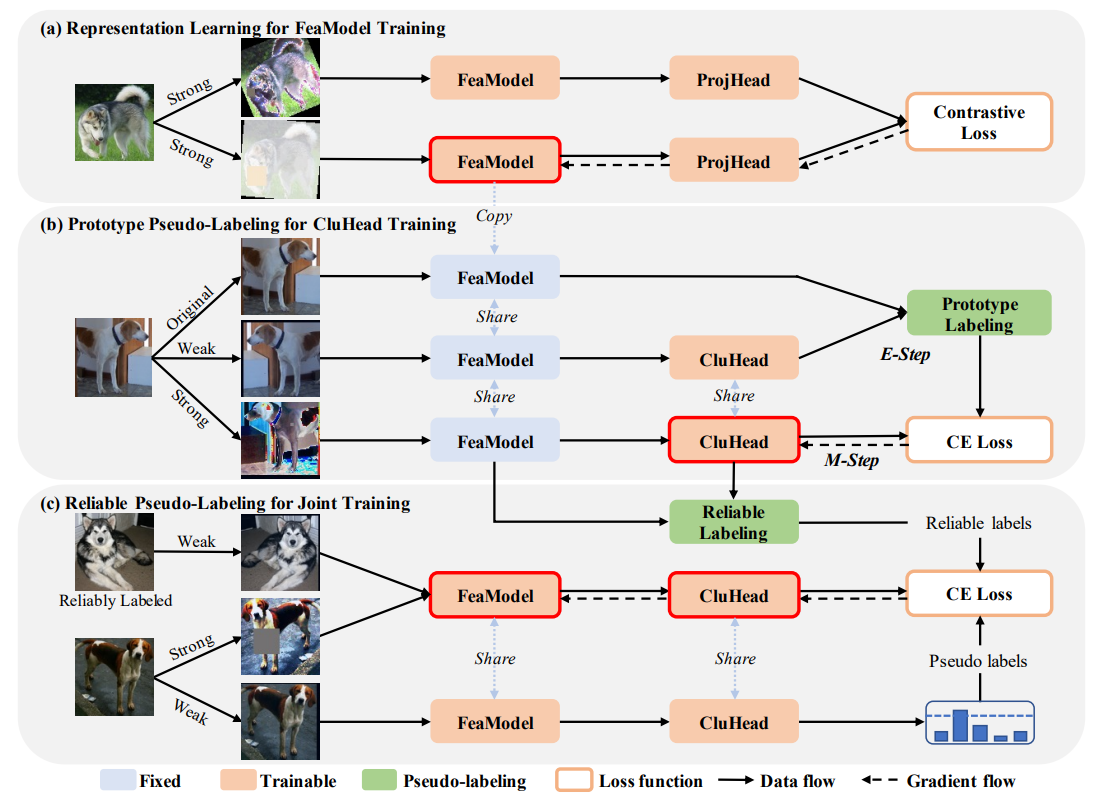
\includegraphics[width=0.8\textwidth]{spice.png}
	\caption{Этапы обучения метода SPICE. 
	FeaModel - энкодер, ProjHead - проекционная голова, CluHead - кластеризационная голова. a) Обучение энкодера. b) Обучение кластеризационной головы.
	с) Совместное обучение энкодера и кластеризационной головы. }
	\label{fig:spice}
\end{figure}

Схематический принцип работы каждого этапа можно видеть 
на Рисунке~\ref{fig:spice}. Перейдем к разбору каждого этапа
по отдельности.

\subsubsection{Обучение энкодера}

Помимо энкодера, будем учить проекционною голову, которая 
представляет из себя двухслойный MLP. Как показано на 
Рисунке~\ref{fig:spice}(a), мы копируем энкодер и 
кластризационную голову, чтобы получить две ветки 
для обучения. На вход веткам подаются разные аугментации 
одного и того же изображения. Далее считается
лосс, максимизирующий косинусную похожесть результатов веток. 
Также лосс минимизирует косинусную похожесть результата 
верхней ветки для текущего сэмпла и негативных примеров. 
В качестве негативных примеров можно взять любые сэмплы 
отличные от текущего.
Градиентный спуск оптимизирует только нижнюю ветку, 
а верхняя обновляется 
как экспоненциально движущееся среднее нижней. 

\textbf{Замечание.} На самом деле вместо описанного 
алгоритма можно использовать любой метод обучения представлений
для изображений без учителя.

\subsubsection{Обучение кластеризационной головы}

Энкодер на этом этапе фиксирован и не обучается. 
На данном этапе у нас есть два набора неизвестных переменных:
оптимальные параметры кластеризационной головы и правильные назначения 
классов объектам. Поэтому для их нахождения мы можем воспользоваться ЕМ-алгоритмом.
На Е-шаге мы считаем параметры кластеризационной головы известными 
и ищем назначения кластеров объектам. На М-шаге мы
считаем известными назначения кластеров и оптимизируем параметры 
кластеризационной головы. Рассмотрим подробно эти 2 шага.

На Е-шаге мы сначала вычисляем признаки $f_i$ из 
верхней ветки Рисунок~\ref{fig:spice}(b). С помощью 
средней ветки мы получаем вероятности каждого кластера для 
каждого объекта из батча. Для каждого кластера мы выбираем 
топ $\frac{M}{K}$ объектов с максимальными 
вероятностями полученными из второй ветки, и берем их признаки
$f_i$ как показано в \ref{eq:prototype_cluster_features}.
\begin{align}\label{eq:prototype_cluster_features}
	\mathfrak{F}_k=\left\{f_i\Big\vert i\in\text{argtopk}\left(P_{:,k}, \frac{M}{K}\right), 
	\forall i=1, \ldots, M \right\}
\end{align}

Здесь $M$ -- это 
размер батча, а $K$ -- количество кластеров задаваемое как 
гиперпараметр до начала работы алгоритма. $P$ -- это матрица
вероятностей, где по строкам разложены вероятности кластеров 
для каждого объекта из батча.

Далее для 
каждого класса $k$ мы вычисляем его центр $\gamma_k$, 
как среднее по точкам из $\mathfrak{F}_k$. Затем 
мы вычисляем косинусную похожесть между признаками $f_i$ 
и центрами кластеров $\gamma_k$. За $\mathfrak{X}^k$ обозначим 
$\frac{M}{K}$ ближайших в данной метрике объектов к 
центру кластера $\gamma_k$. Скажем что все объекты 
в $\mathfrak{X}^k$ имеют одну и туже псевдометку, а именно 
$y_i^s=k\quad \forall x_i\in\mathfrak{X}^k$. Результатом 
E-шага будет следующее множество пар объект-псевдометка:
\[
	\mathfrak{X}^s=\{(x_i, y_i^s)\mid \forall x_i 
	\in \mathfrak{X}^k, k=1,\ldots, K \}
\]

Будем называть псевдометки из $\mathfrak{X}^s$ протопсевдометками.

Перейдем к M-шагу. Используя протопсевдометки с Е-шага и вероятности 
классов, полученные из нижней ветки, мы можем посчитать следующую функцию 
потерь:
\[
	\mathcal{L}_{clu}=\frac{1}{M}\sum_{i=1}^M L_{ce}(y_i^s, p_i')
\]

Здесь $L_{ce}$ -- логистическая функция потерь, $p_i'=\text{softmax}(p_i)$. 
$p_i$ -- это вероятности полученные из нижней ветки. Стоит отметить, что в итоге к 
логитам из нижней ветки дважды применяется операция softmax. Авторы 
объясняют такое решение тем, что двойной softmax замедляет процесс обучения. 
Таким образом, такая функция потерь меньше доверяет протопсевдометкам, 
что особенно полезно в начале обучения. 

Функция потерь $\mathcal{L}_{clu}$ используется для прохода назад 
через кластеризационную голову. Затем делается шаг градиентного спуска.

Можно заметить, что 2-ой этап довольно легковесный, так как нам необходимо 
обучать только кластеризационную голову с малым количеством параметров. 
Поэтому авторы предлагают параллельно учить сразу несколько голов и выбирать
лучшую по функции потерь $\mathcal{L}_{clu}$ для уменьшения дисперсии решения.

Стоит также обратить внимание, что распределения аугментаций 
для разных веток отличаются. Как видно на рисунке \ref{fig:spice}(b) 
верхней ветке на вход подается оригинал изображения, средней ветке
слабо аугментированое изображение, а нижней сильно аугментированное.

\subsubsection{Совместное обучение энкодера и кластеризационной головы}

На данном этапе мы хотим дообучить энкодер и кластеризационную голову.
Для этого мы говорим, что у сэмпла $x_i$ псевдометка $y_i^s$ 
надежная, если среди $N_s$ ближайших по косинусной похожести 
соседей к $x_i$ доля объектов, имеющих такую же псевдометку, 
больше порога $\lambda$. $N_s$ и $\lambda$ -- гиперпараметры.

В дальнейшем надежные метки фиксируются и не меняются 
все время обучения. В некотором смысле их можно считать 
настоящими метками. Поэтому для обучения энкодера и 
кластеризационной головы можно использовать любой 
алгоритм частичного обучения. Авторы SPICE использовали метод
FixMatch \cite{NEURIPS2020_06964dce}.

\subsection{TEMI}

Метод кластеризации изображений TEMI \cite{Adaloglou_2023_BMVC} 
использует в качестве энкодера модель, 
предобученную без учителя, для получения представлений изображений. 
Сама статья описывает способ обучения ансамбля из кластеризационных голов.

\subsubsection{PMI}

Будем считать что изображение $x\in\mathcal{X}$ это случайная 
переменная из распределения с плотностью $p(x)$.
Пусть $p(c)$ это вероятность того что $x$ имеет 
класс $c\in\{1, \ldots, C\}$. За $p(x, x')$ обозначим 
вероятность того, что изображения 
$x$ и $x'$ имеют один и тот же класс. Легко видеть, что 
$p(x, x')=\sum_{c=1}^{C}p(x|c)p(x'|c)p(c)$. Введем 
$q(c|x)$, который будет нашим обучаемым классификатором, 
сообщающим вероятность класса $c$ для картинки $x$. 
Используя формулу Байеса, получаем $q(x|c)=
q(c|x)p(x)/q(c)$. Тогда можно аппроксимировать 
$p(x, x')$ следующим образом:

\[
	q(x, x')=\sum_{c=1}^C q(x|c)q(x'|c) q(c).
\]
Теперь определим \textit{поточечную взаимную информацию} (PMI)
как:
\[
	\text{pmi}(x, x') \defeq \log \frac{q(x, x')}{p(x)p(x')} = 
	\log \sum_{c=1}^C \frac{q(c|x)q(c|x')}{q(c)}
\]

Оказывается, что наилучший классификатор $q^{\ast}(c|x)$, 
т. е. совпадающий с $p(c|x)$ во всех точках $x$ с 
точностью до перестановки индексов кластеров, 
это классификатор, максимизирующий матожидание $\text{pmi}(x, x')$.
Отметим, что выполнение этого свойства гарантируется только 
в случае вырожденного распредления $p(c|x)$, т. е. когда 
каждому изображению соответствует ровно 1 класс.

\subsubsection{Самодистиляция}

Обозначим энкодер за $g$ и найдем для каждого изображения 
$x$ его представление $g(x)$. В полученном признаковом пространстве 
найдем для каждого объекта $x$ k ближайших соседей по косинусной похожести и
обозначим их за $S_x$. Во время обучения мы будем брать случайный 
$x$ из датасета и случайный $x'$ из $S_x$. Предполагается, что 
$x$ и $x'$ будут в одном кластере с большой вероятностью. 

Введем две кластеризационные головы: студента $h_s(\cdot)$
и учителя $h_t(\cdot)$. Каждая из голов это трехслойная 
полносвязная сеть. Чтобы получить $q_s(c|x)$ и $q_t(c|x')$ 
используем софтмакс с температурой $\tau$ на логитах 
$h_s(g(x))$ и $h_t(g(x'))$ соответственно. 

Аппроксимируем PMI следующим образом:
\[
	\widetilde{\text{pmi}}(x, x') \defeq \log 
	\sum_{c=1}^C \frac{(q_s(c|x)q_t(c|x'))^{\beta}}{\tilde{q}_t(c)}
\]

Гиперпараметр $\beta\in(0.5, 1]$ помогает 
избегать вырожденных решений, делая вклад крупных кластеров 
менее важным. $q(c)$ оценим экспоненциально движущимся средним:

\[
	\tilde{q}_t(c)\leftarrow m \tilde{q}_t(c) + 
	(1-m)\frac{1}{B}\sum_{i=1}^B q_t(c|x_i)
\]
где B это размер батча, $m\in(0, 1)$ гиперпараметр инерции.

Чтобы получить лосс нужно взять $\widetilde{\text{pmi}}(x, x')$ 
со знаком минус и симметризовать его:
\[
	\mathcal{L}(x, x') \defeq 
	-\frac{1}{2}\left(\widetilde{\text{pmi}}(x, x') 
	+\widetilde{\text{pmi}}(x', x)\right)
\]

Параметры $h_s(\cdot)$ оптимизируются градиентным спуском, 
в то время как параметры $h_t(\cdot)$ это экспоненциально 
движущееся среднее параметров головы студента.  

\subsubsection{Взвешивание пар}

Так как не все пары соседей $x$ и $x'$ будут иметь 
один класс, введем вес, позволяющий уменьшить вклад 
ложноположительных пар в лосс:
\[
	w(x, x')=\sum_{c=1}^C q_t(c|x)q_t(c|x')
\]

Также мы будем учить не одну пару голов, а сразу 
$H$ пар. Причем для каждой головы для взвешивания 
пары будем использовать веса, полученные из всех голов. 
Таким образом, финальный лосс для $i$-ой пары голов выглядит 
так:
\[
	\mathcal{L}_{\text{TEMI}}^i(x, x')\defeq 
	\frac{1}{H}\sum_{j=1}^H w_j(x, x')\mathcal{L}^i(x, x')
\]

\subsection{Обучение представлений}

Как уже было упомянуто раннее, первый шаг для кластеризации
сложных объектов -- это извлечение хороших признаков из объекта.
Существует множество методов, которые нацелены именно на эту задачу.

Один из примеров это фреймворк BYOL \cite{NEURIPS2020_f3ada80d}.
Он учит представления для изображений без учителя в предположении,
что признаки для двух аугментаций изображения должны быть 
в некотором смысле похожи. А именно, проекция признаков для 
одной аугментации должна иметь как можно большую косинусную 
похожесть с проекцией признаков другой аугментации, к которой 
применили MLP.

\subsection{Случай аудио}

Рассмотренные раннее методы занимаются кластеризацией 
изображений. Однако их можно адаптировать для кластеризации 
аудио. Для этого каждую аудиозапись можно преобразовать в 
изображение, отражающее ее структуру -- спектрограмму.
Так например DeepCluster был адаптирован для аудио как 
DECAR \cite{Ghosh2022DECARDC}.

Аналогичным образом BYOL был адаптирован для аудио как 
BYOL-A \cite{BYOL_A}. Важным отличием от классического
BYOL является наличие специфичных для аудио аугментаций.
Например используется аугментация Random Linear Fader, 
которая моделирует эффект приближения/удаления источника
звука.

Еще один интересный пример получения представлений 
для аудио это wav2vec 2.0 \cite{NEURIPS2020_92d1e1eb}. 
Он работает с аудио как с последовательностью и кодирует 
её с помощью трансформера. Чтобы получить представление 
для всего аудио в целом, можно к примеру усреднить полученную
последовательность представлений. 

Существуют также методы обучения с учителем 
представлений для аудио. Примером может служить 
PaSST \cite{Koutini2021EfficientTO}. Он разбивает 
спектрограмму на патчи, которые передаются в трансформер. 
Чтобы ускорить обучение в трансформер подаются не все 
патчи, а только их часть. Как оказывается такой подход не 
только ускоряет обучение, но и является техникой регуляризации,
улучшающей качество.

\section{Бейзлайн}

Для получения бейзлайна будем использовать тройки: 
энкодер, метод понижения размерности, классический 
метод кластеризации. Сначала аудиозаписи проходят 
через энкодер превращаясь в векторы признаков. 
Затем полученные эмбеддинги уменьшаются с помощью метода
понижения размерности. Наконец, к сжатым эмбеддингам 
применяется классический алгоритм кластеризации. 
В качестве метрик качества используются NMI и доля 
правильных ответов.

Для понижения размерности используются PCA \cite{PCA_overview} и 
t-SNE \cite{JMLR:v9:vandermaaten08a}. Для кластеризации 
используются K-means, DBSCAN \cite{ester1996density}, 
MeanShift \cite{fukunaga1975estimation}, Agglomerative 
clustering \cite{agglomerative}.

В качестве датасета было использовано подмножество 
датасета DCASE 2018 task 5\footnote{\url{https://dcase.community/challenge2018/task-monitoring-domestic-activities}}.
В нем собраны аудиозаписи активности человека проживающего в 
отеле на протяжении одной недели. Всего классов 9. 

Результаты можно видеть в Таблице~\ref{table:baselines}. 
Стоит отметить, что помимо предобученной BYOL-A мы 
также замеряем её качество со случайной инициализацией 
весов, что отражено в таблице как Random BYOL-A.
\begin{table}[]
    \footnotesize
	\centering
\begin{tabular}{lllll}
\toprule
Features producer & Dimensionality reducer & Clustering method &   NMI    &    accuracy    \\
\midrule
BYOL-A & None & AgglomerativeClustering &  \textbf{0.64} &      \textbf{0.68} \\
         &      & K-means &  0.60 &      0.64 \\
         & PCA & AgglomerativeClustering &  \textbf{0.64} &      0.66 \\
         &      & DBSCAN &  0.55 &      0.52 \\
         &      & K-means &  0.59 &      0.61 \\
         &      & MeanShift &  0.54 &      0.54 \\
         & t-SNE & AgglomerativeClustering &  0.62 &      0.63 \\
         &      & K-means &  0.61 &      0.61 \\
         &      & MeanShift &  0.54 &      0.51 \\
\midrule
Random BYOL-A & None & AgglomerativeClustering &  0.57 &      0.60 \\
         &      & K-means &  0.55 &      0.60 \\
         & PCA & AgglomerativeClustering &  \textbf{0.60} &   \textbf{0.67} \\
         &      & DBSCAN &  0.48 &      0.51 \\
         &      & K-means &  0.56 &      0.62 \\
         &      & MeanShift &  0.46 &      0.52 \\
         & t-SNE & AgglomerativeClustering &  0.57 &      0.61 \\
         &      & K-means &  0.55 &      0.59 \\
         &      & MeanShift &  0.27 &      0.44 \\
\midrule
PaSST & None & AgglomerativeClustering &  0.68 &      0.71 \\
         &      & K-means &  0.59 &      0.57 \\
         & PCA & AgglomerativeClustering &  \textbf{0.69} &       \textbf{0.72} \\
         &      & DBSCAN &  0.51 &      0.54 \\
         &      & K-means &  0.60 &      0.65 \\
         &      & MeanShift &  0.45 &      0.51 \\
         & t-SNE & AgglomerativeClustering &  0.65 &      0.69 \\
         &      & K-means &  0.61 &      0.59 \\
         &      & MeanShift &  0.63 &      0.69 \\
\midrule
wav2vec2 & None & AgglomerativeClustering &  0.33 &      0.40 \\
         &      & K-means &  0.32 &      0.43 \\
         & PCA & AgglomerativeClustering &  0.33 &      0.46 \\
         &      & DBSCAN &  0.31 &      0.47 \\
         &      & K-means &  0.33 &      0.43 \\
         &      & MeanShift &  0.15 &      0.39 \\
         & t-SNE & AgglomerativeClustering &  0.34 &      0.39 \\
         &      & K-means &  \textbf{0.36} &      0.39 \\
         &      & MeanShift &  0.35 &      \textbf{0.58} \\
\bottomrule
\end{tabular}

	\caption{Сравнение энкодеров, методов уменьшения размерности и методов кластеризации.
	Жирным шрифтом выделены лучшие значения метрик для каждого энкодера.}
	\label{table:baselines}
\end{table}

\section{План дальнейшей работы}

В дальнейшем планируется адаптировать методы SPICE и TEMI для аудио.
Планируется измерить для 
полученных методов метрики NMI и долю правильных ответов на том же
датасете, который использовался для оценки бейзлайна. Затем планируется 
сравнить полученные метрики с 
бейзлайном и сделать выводы. 
	
\newpage 
\printbibliography[heading=bibintoc] 
	
\end{document}
